\documentclass{article}
\usepackage[utf8]{inputenc}

\title{Literature Review}
\author{Kent Alejandro Rush }
\date{November 2019}

\usepackage{natbib}
\usepackage{graphicx}

\begin{document}

\maketitle

\section{Introduction}

Light curves are data collected by observing the brightness of an object as it passes over an observer. This data has been used in astronomy to determine properties of asteroids and other celestial bodies. The focus of this paper will be to take these analysis methods and instead apply them to light curves gathered from earth-orbiting spacecraft. Potential applications of this data include spacecraft health monitoring, determination of optical properties, geometry, selecting targets for space debris removal, and determining the mission of an unknown spacecraft. An example light curve can be seen in figure \ref{lightcurve_im}.

\begin{figure}[h]
	\centering
	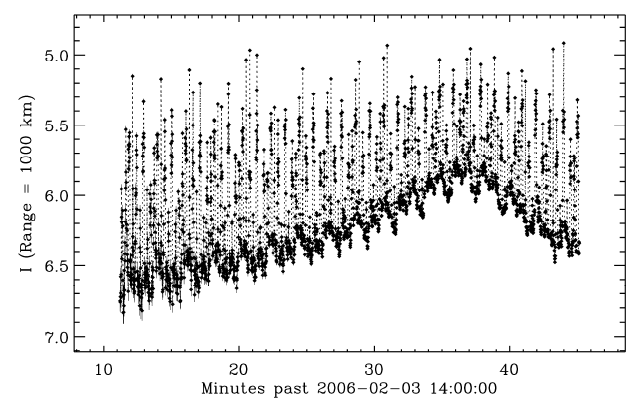
\includegraphics[width=0.5\textwidth]{lightcurve_AMOS}
	\caption{Lightcurve of the IMAGE spacecraft \cite{AMOS}.}
	\label{lightcurve_im}
\end{figure}

Light curve analysis has been applied to natural celestial bodies such as planets and asteroids long before it was applied to artificial satellites. Many of the methods and techniques developed to extrude information from satellite light curves have been derived from methods previously applied to asteroids with general success. The notable differences between asteroids and artificial satellites are geometry, albedo and perturbations \cite{Separating}. Spacecraft, unlike asteroids are characteristically non-convex, have large variations of albedo across their surfaces due to their varied materials, and are more affected by perturbations from their environment because of their smaller mass. Additionally, functioning spacecraft are usually controlled. This requires more complex models to determine a spin axis.

While the techniques derived from astronomy have had some success, they do not answer all of the possible spacecraft related questions we might want answered. These questions have to do with orbit, mass, and attitude determination among others. For these, formulations of the Kalman Filter have been proposed which combine a models of how the spacecraft should behave and the way it should reflect light, and compare them to actual measured data. 

This paper presents a synthesized review on the topic of light curve analysis with respect to spacecraft.

\section{Literature Review}

\subsection{Period Estimation}

The most fundamental form of light curve analysis is determining the period of a body rotating about its major axis. One of the most influential publications on this topic was written by Hall et al.\cite{AMOS} where the spin rate and spin axis were able to be determined for the defunct AMOS spacecraft. The state of being in rotation about its major axis is important because this state is in stable equilibrium, and the angular velocity can be assumed to be constant in inertial space. This assumption allows for a solution to be found, but does not hold for spacecraft which are tumbling chaotically.

Period estimation can be broken up into two principal steps: Determining synodic, then the sidereal period. The synodic period refers to the period of the spacecraft as viewed from earth. Due to the earths rotation, the synodic period is the non-inertial period between the spacecraft and the observer. The sidereal period is the absolute rotation period in inertial space and is the more useful of the two measurements. 

\subsubsection{Synodic Period}

The most common way to calculate the synodic period is to conduct spectral analysis using the Fourier transform or Lomb-Scargle periodogram. For these methods to work, it needs to be assumed that the object is spinning about its major axis. This assumption has served the astronomical community well considering that most celestial bodies have had eons to settle into their minimum energy states. Spacecraft, however, have not had eons, and are potentially tumbling chaotically \cite{AMOS}. Alternate methods such as using two-dimensional Fourier transforms for spacecraft exhibiting multi-axis rotation has been investigated by Hall et al.  and a Kalman filter approach by  Wetterer C et. al. demonstrated the ability to converge to similar results without assuming major axis rotation \cite{Hall2014OpticalCO} \cite{AttitudeEstimationFromLightCurve}. A plot of the synodic perdiod of the IMAGE spacecraft during a pass can be seen in figure \ref{synodic_im}

\begin{figure}[h]
	\centering
	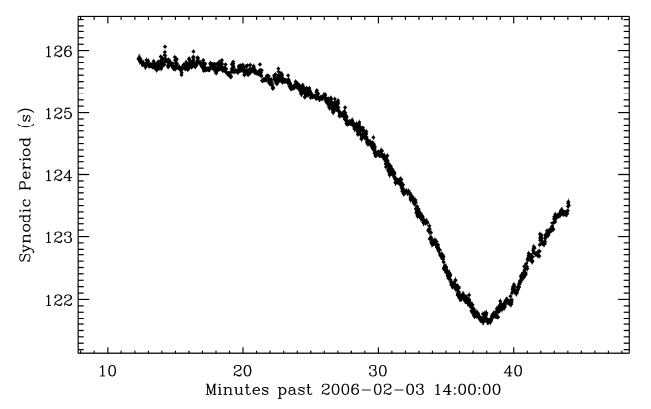
\includegraphics[width=0.5\textwidth]{synodic_period_AMOS}
	\caption{Measured synodic period of the IMAGE spacecraft \cite{AMOS}.}
	\label{synodic_im}
\end{figure}

A large component of typical synodic period analysis is transforming the light curve into the frequency domain. Typically, a Fourier transform is applied and the peak frequency is interpreted to be the synodic period. However, a known drawback of the Fourier method is that it requires evenly spaced data which is not easily attained in practical applications. This can be solved by interpolating between data points, at the cost of adding significant noise to the measurements \cite{Tagliaferri}. Because of this, the Lomb-Scargle periodogram method is commonly applied to unevenly spaced light curve data. Recently, investigations into neural networks for spectral analysis have been conducted by Tagliaferri et al. have demonstrated their ability to outperform the Fourier transform and lomb-scargle method using data sets that are unevenly spaced \cite{Tagliaferri}.

Another serious drawback to frequency analysis of light curves is the sampling frequency limitation. It is only possible to measure a spin rate with a frequency that is less than half of the sampling frequency due to the Nyquist sampling criterion \cite{SILHA2018844}. This poses a fundamental limitation to all frequency based analysis and is dependent on the measurement hardware. 

Oftentimes, a one-dimensional Fourier transform fails to describe the motion of a spacecraft which suggests indicate that the spacecraft is tumbling chaotically or is rotating about two axes in a coning motion \cite{Hall2014OpticalCO}. In the case that a spacecraft is rotating along two axes in a coning motion, a two-dimensional Fourier transform has been proposed as a method to determine the rotation state.

\subsubsection{Sidereal Period}
After the synodic period is determined, there exist multiple methods for calculating the sidereal period. By far the most popular seems to be the Epoch Method. Remarkably, this method requires no prior knowledge of the spacecrafts geometry and can determine the spin axis of the spacecraft assuming that it is spinning about its major axis. 

The fundamental assumption of the Epoch Method is that the synodic period is related to the motion of the Principal Axis Bisector (PAB, see figure \ref{PAB_im}) about the spin axis of the spacecraft. The PAB is defined to be the normalized mean vector between the sun and observation vectors. The second assumption is that the spacecraft is spinning about its major axis. Again, the major axis assumption is so that the angular velocity vector can be assumed to be constant in inertial space.

\begin{figure}[h]
	\centering
	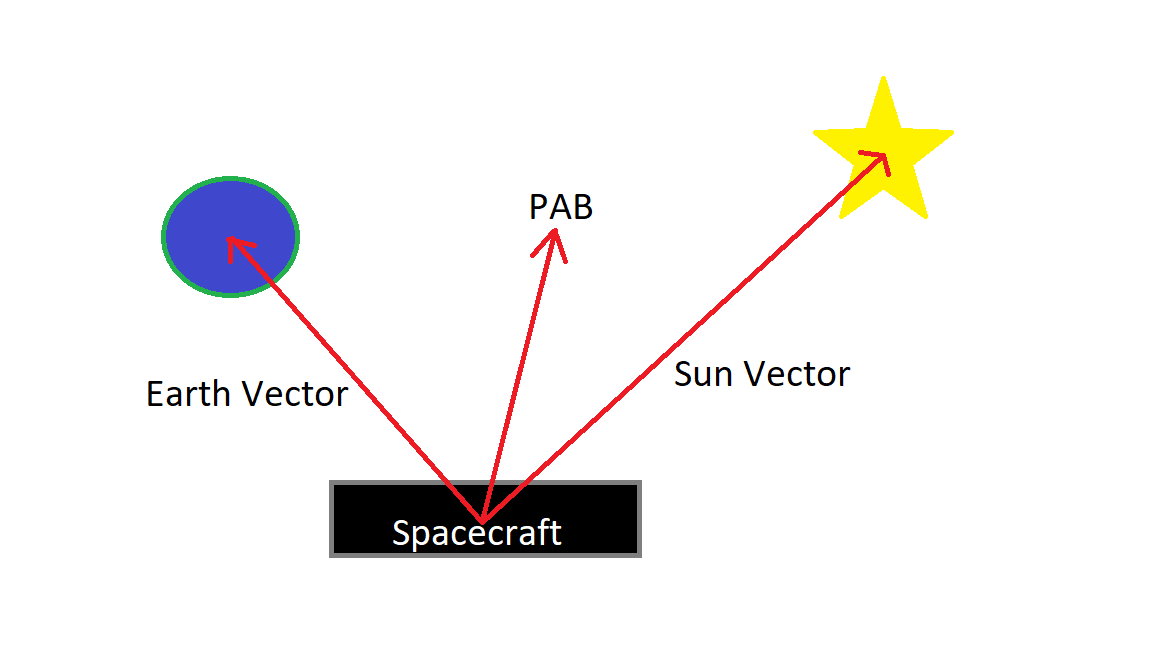
\includegraphics[width=0.5\textwidth]{PAB}
	\caption{Principal Axis Bisector (PAB).}
	\label{PAB_im}
\end{figure}

The fundamental principle of the epoch method is that as an object passes an observer, its observed synodic period changes over time. So, for any given spin axis, there is a sidereal period that most accurately predicts the measured changes in synodic period. The algorithm then, is to conduct a grid search through the space of possible spin axes and return the spin axis whose set of predicted synodic periods best fits the measured data. The results of a grid search can be seen in figure \ref{epoch_grid_search_im}

\begin{figure}[h]
	\centering
	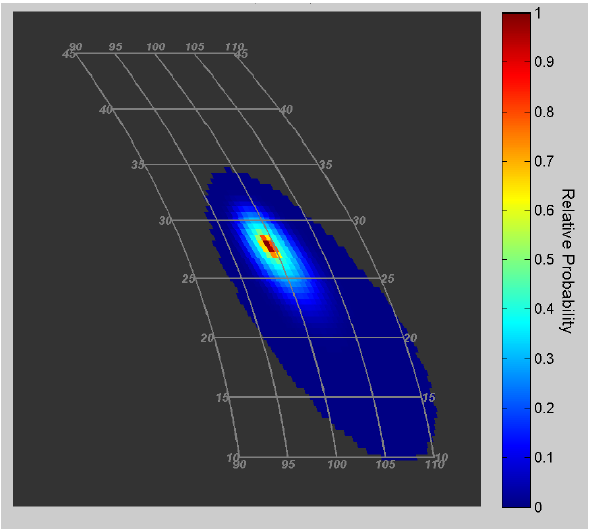
\includegraphics[width=0.5\textwidth]{spin_axis_OPTICAL_CHARACTERIZATION}
	\caption{spin axis distribution for the D4S2 rocket-body \cite{Hall2014OpticalCO}.}
	\label{epoch_grid_search_im}
\end{figure}

It is important to notice that it is change in the synodic frequency across an observation that allows the Epoch Method to converge on an optimal solution \cite{Wallace}. For this modulation to occur, the PAB must change sufficiently quickly during the observation. This condition is satisfied well for spacecraft in low earth orbit. However, this can be problematic for deep space and geostationary spacecraft.

Another method used by astronomers to determine sidereal period and pole orientation is the Amplitude-Magnitude method which works on the idea that variations in brightness are caused by a changing projected surface area \cite{Magnusson1989DeterminationOP}. This technique has been applied to asteroids which can be assumed to be tri-axial ellipsoids as it is possible to determine the relative size of each axis from amplitude-longitude and magnitude-amplitude plots which are generated by observing the asteroid at different oppositions \cite{Magnusson1989DeterminationOP}. 

After the relative geometry has been determined, it is possible to calculate the angle between the observers line of sight and spin axis (aspect angle), creating a circle of possible spin vectors. By combining the "aspect circles" from multiple measurements it is possible to converge on two spin vectors which best fit the points of intersection of these circles \cite{Magnusson1989DeterminationOP}. This technique could be applied to the analysis of rocket bodies or other spacecraft that are generally ellipsoidal in shape, however this technique has not yet been applied to spacecraft.



A third method proposed by Wallace et al.  is an algorithm that uses the glints (brief flashes) caused by flat surfaces on a spacecraft as they present themselves normal to the PAB \cite{Wallace}. The way this algorithm works is by assuming sidereal frequency and spin axis which are fed into a model that predicts glint times. The algorithm then finds the combination of sidereal spin rate and spin axes that minimize the difference between the observed and measured glint times. Again, for this method to work the object must be assumed to be spinning about its major axis.

Unfortunately, this method requires sufficient knowledge of the spacecrafts geometry that a simplified model can be created. For identified and documented spacecraft this can be acquired; however, for pieces of space debris and unidentified spacecraft it is not possible to apply this method.

A minor problem with all of the above techniques that determine spin axis is that it is impossible to determine whether the spacecraft is rotating clockwise or counterclockwise around the spin vector \cite{Magnusson1989DeterminationOP}.

\subsection{Light Curve Inversion}

Light Curve Inversion (LCI) is a technique developed by M. Kaasalainen et. al. to estimate the shape of asteroids \cite{KAASALAINEN2002369}. Essentially, this process generates a set of facet normal unit vectors and assigns each an albedo-area (the product of albedo and area). Using these normals and albedo-areas, a lightcurve can be simulated using simple models. Using the difference between the simulated lightcurve and the acutal data, the albedo-areas for each facet normal can be optimized to best fit the data \cite{Kaasalainen}. Once a set of facet normals and corresponding albedo-areas has been converged upon and if the albedo values are known or assumed, one can solve to Minkowski Minimization problem which will yield a unique convex polyhedron \cite{Minkowski1989}.

In order to generate a light curve from the estimated geometry, the orientation of the body has to be known \cite{PSI}. While an arbitrary body frame can be assigned to the body, the angular velocity of the body must be known in order to propagate the orientation of this frame through the simulation. This generally limits the application of this technique to objects spinning about their major axis and whose angular velocity magnitude and direction can be calculated using the aforementioned Epoch method. However, as long as the angular velocity is known there is no reason why this method cannot be applied.

Another limitation is that any light curve can be explained by any combination of geometry and albedo \cite{Magnusson1989DeterminationOP}. For asteroids this can be dealt with by assuming a constant albedo across the entire surface. This assumption does not hold for an unknown spacecraft which may be composed of dozens of materials with different albedos. For shape determination of spacecraft albedo values need to either be known or assumed. 

Work by Calef et al. demonstrates that by combining data from reflections as well as thermal emissions, it is possible to separate the effects of geometry, albedo, and emissivity \cite{Separating} \cite{PSI}. 

It is also worth mentioning that, while insufficient to determine shape on its own, the albedo-area distribution is a complete description of the body parameters of a convex shape linking attitude to radiant intensity \cite{Separating}.

The final biggest limitation of LCI is that it can only generate convex hulls, which most asteroids are but most spacecraft are not. Still, there are many spacecraft whose shape overall is convex, and the convex hull of a concave spacecraft still contains useful information. Estimating non-convex geometries has had limited success, the issues being that many local minimums exists which pose an issue for error minimizing techniques \cite{Kaasalainen}. The results of a convex hull estimation on a box-wing spacecraft can be seen in figure \ref{shape_im}.

Despite these limitations there has been limited success in determining the shapes of rocket bodies and cubesats in simulation by Bradley et al \cite{Bradley2014LIGHTCURVEIF}.

\begin{figure}[h]
	\centering
	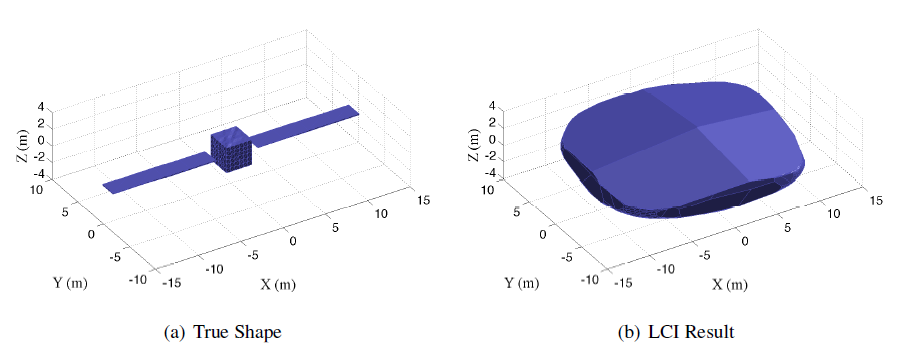
\includegraphics[width=1\textwidth]{lci_LIGHTCURVE_INVERSION}
	\caption{Light Curve Inversion of a box-wing satellite \cite{Bradley2014LIGHTCURVEIF}.}
	\label{shape_im}
\end{figure}

\subsection{Phase-Angle Brightness Comparisons}

Another method of estimating a spacecraft's shape is to compare the Phase-Angle Brightness plots of the measured spacecraft with that of a known geometry \cite{Separating}. A Phase-Angle Brightness graph simply shows the distribution of reflected intensity against the phase-angle of the measurement. By comparing with either simulated data from a known geometry or with data from observations of a known spacecraft, one can infer the similarity between geometries. Example brightness plots can be seen in figure \ref{phase_angle_bright_im}.

\begin{figure}[h]
	\centering
	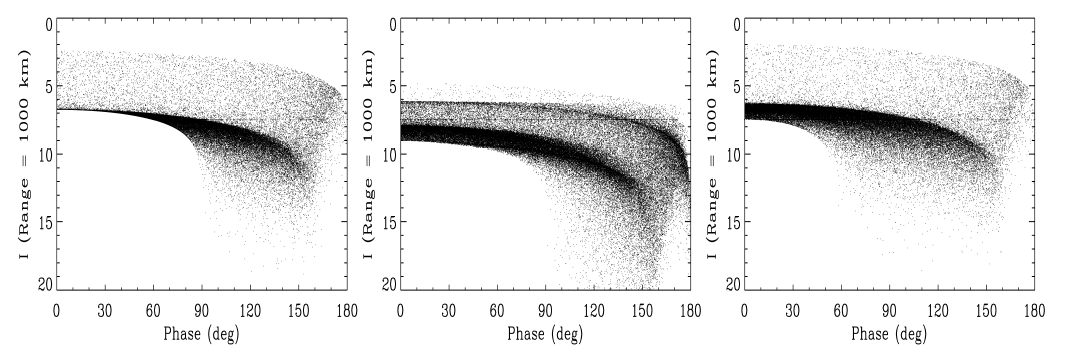
\includegraphics[width=\textwidth]{phase_angle_brightness_SEPARATING_ATTITUDE}
	\caption{Simulated Phase Angle Brightness plots \cite{Separating}.}
	\label{phase_angle_bright_im}
\end{figure}

\subsection{Applications of the Kalman Filter}

Kalman Filters excel at estimating parameters when a model and data can be corroborated. Since the models for orbital dynamics, spacecraft rotation, and reflection are all well known, it is no surprise that the Kalman Filter has been applied extensively in this area.

\subsubsection{Attitude Estimation}
One of the most common applications of Kalman filtering when applied to light curve data is to estimate the attitude and rotation of a spacecraft given a known geometry \cite{AttitudeEstimationFromLightCurve} \cite{LINARES20141} \cite{SpaceObjectCharacterization}. These filters work by guessing an initial attitude and angular velocity and generating a reflectance value based on the known obit and material properties of the spacecraft model. The Kalman filter performs this operation across the entire dataset, comparing the predicted reflectance intensities with the measured data and updating its estimate of the spacecraft's attitude and angular velocity. Eventually this method should converge to an state representation of the spacecraft that matches the measured data as closely as possible.

\begin{figure}[h]
	\centering
	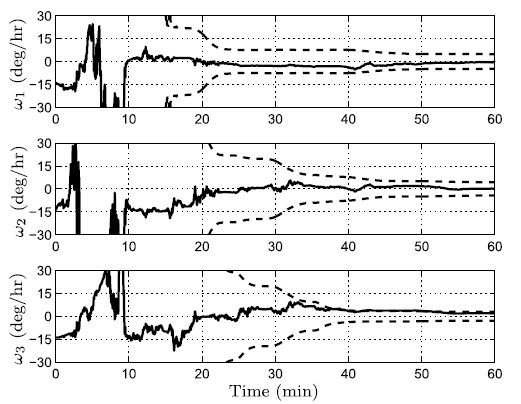
\includegraphics[width=.5\textwidth]{Kalman_convergence}
	\caption{Convergence of angular velocity estimate using Kalman filters \cite{SpaceObjectCharacterization}.}
	\label{ukf_convergence_im}
\end{figure}

Several formulations have been proposed, each estimating different quantities but all estimating attitude and angular velocity. It is interesting to note that while the Kalman filter formulation by Wetterer et al. assumed a constant angular velocity, Linares et al. and Linares et al. both used a fomulation that allowed for a changing angular velocity \cite{AttitudeEstimationFromLightCurve} \cite{LINARES20141} \cite{SpaceObjectCharacterization}. However, in all of their test cases they used spacecraft that were spinning about their major axis.

In order to account for a variable spin axis, information about the inertia of the spacecraft is required. If the geometry is known, assumptions of the distribution of mass can be made, and a crude estimate of the spacecraft's inertia can be made \cite{LINARES20141}.

It has been demonstrated through simulation that by using Kalman filters it is possible to converge on usefully accurate values for attitude and angular velocity as well as other parameters, see figure \ref{ukf_convergence_im}. Of the papers read in this review, only Wetterer et al. attempted to apply their techniques to real data. Their attempt proved unsuccessful and cited difficulties due to their simplified reflectance model and simplified geometric model of the rocket body \cite{AttitudeEstimationFromLightCurve}.


\subsubsection{Shape Characterization}

Using the same principles as above, it is possible to guess a geometry and see how well it is capable of fitting the data. Linares et al. demonstrated success in running multiple Kalman filters in parallel and applying a multiple-model adaptive estimation(MMAE) algorithm to select the geometry with the best fit \cite{SpaceObjectCharacterization}. Since many spacecraft have similar geometries, this method shows promise for determining a non-convex geometry for a completely unknown spacecraft. The downside is that there is no guarantee that the true geometry is within the set of hypothesized geometries. However, should the true geometry be in the set of hypothesized geometries, this process will select it and allow for the analysis conducted by \cite{AttitudeEstimationFromLightCurve}. This would be exciting because it would allow for the determination of the angular velocity of a chaotically spinning, unknown spacecraft.

\subsubsection{Angles and Light Curve Synthesis}

Going one step beyond simply estimating the spacecraft attitude and angular velocity, it is possible to synthesize light curve data with other data to estimate parameters that are not directly measurable such as the mass of a spacecraft.

R. Linares et. al  and M. Jah. et. al. demonstrated that by using a Kalman filter to sythesize light curve data with angular observation measurement (angles) it is possible to estimate the mass, area, and albedo of a spacecraft as well as its orbital state vectors \cite{LINARES20141} \cite{StateAndParameter}. Their method models the effects of solar radiation pressure (SRP) and aerodynamic drag on the orbit and compares the predicted changes to the perturbations measured by the angles data. 

\subsection{Light Curve Simulation}

In order to determine the spin axis and spin rate of an object spinning about its major axis, only the measured light curve data is needed. However, for the majority of further analyses that have been proposed, the ability to generate a light curve from a spacecraft model is necessary. For shape, attitude, optical property, etc., these parameters are converged upon by minimizing the error between a simulated light curve and actual, measured data. Many applications utilize simplified reflectance models and are only verified through simulation. In order to apply these methods to real data, it is necessary to implement higher fidelity models \cite{AttitudeEstimationFromLightCurve}.

Simulating a light curve requires three components: a scattering law, also referred to as a bi-directional reflectance distribution function (BRDF), a model of the spacecraft, and a ray tracing algorithm. The third is only necessary if the spacecraft model is non-convex, as it is only used to deal with the issue of self-shading geometry \cite{Kaasalainen}. The scattering law is the simplest component, which is simply a function of the observation and illumination vectors as well as the optical parameters of the facet being illuminated. The observation vector is the direction from which the object is viewed and the illumination vector is the direction of the sun.

Some of the simplest scattering laws are the Lamberts and Lommel-Seeliger laws. These are little more than cosine laws, decreasing the surface brightness with the cosine of the angles between the observation and illumination vectors and only accounds for albedo \cite{Kaasalainen} \cite{Bradley2014LIGHTCURVEIF}. This is useful for quick simulation, but more commonly the Phong BRDF model is used for spacecraft light curves \cite{StateAndParameter} \cite{SpaceObjectCharacterization} \cite{LINARES20141}. The Phong model is advantageous because it allows for the modeling of diffuse and specular reflection, which allows for differentiation between materials, obeys conservation of energy, and accounts for the changing effects of diffuse and specular reflections as the angle of incidence changes \cite{Ashikhmin}. The differences between these reflectance models can be seen in figure \ref{brdf_comparisons_im}.

\begin{figure}[h]
	\centering
	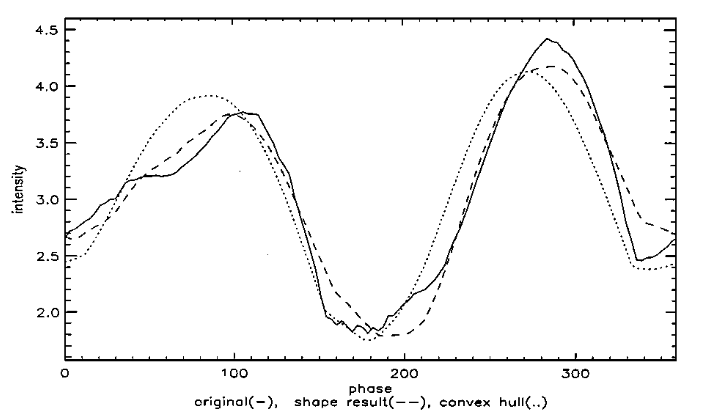
\includegraphics[width=.5\textwidth]{lightcurve_simulation}
	\caption{Comparisons between "true" and simulated light curves of shape estimates using a combination of Lamberts and Lommel-Seeliger laws \cite{Kaasalainen}.}
	\label{brdf_comparisons_im}
\end{figure}

In terms of spacecraft modeling, most researchers choose to use simplified models that represent the spacecraft as a convex shape in order to avoid the need for ray tracing. Since most researchers only validate their studies in simulation, their "truth" data is also generated from a simulation of a convex geometry. Real spacecraft, however, are generally non-convex and can only be approximated by a concave geometry. For applications of Kalman Filters, whose perormance is highly dependant on an accurate measurement function, simulating non-convex geometries with a ray tracing algorithm should improve performance.


\section{Takeaways and Conclusions}

Overwhelmingly, the trend in the research is to perform analysis on spacecraft that are spinning about their major axis. This assumption is valid for many simple, well known, and well studied objects, but limits the utility of analysis to a small subset.

With the applications of Kalman filtering to light curve data, the ability has arisen to determine the spin axis of unresolved spacecraft without assuming a spin about the major axis. This is possible because with a model of the spacecraft it is possible to remove ambiguities in the reflectance data and converge on a changing angular velocity that most closely matches real measurements.

While the more simple analysis techniques like the Epoch and Amplitude-Magnitude methods have been applied successfully to real data, it is not the case for the more complex analyses. For the majority of proposed Kalman filtering and shape estimation algorithms out there, very few have been applied to real data. Wetterer et al. attempted to do so but with no success \cite{AttitudeEstimationFromLightCurve}. This is significant because many researchers so far have validated their results using simulated data which was generated using simplified spacecraft and reluctance models that are not significantly more complex than the approximations used in their analysis. This proves their concepts in theory, but there is still a rift between their work and any practical applications.

The inability to determine a changing angular velocity and the few attempts to apply techniques to real data are the two largest areas of work identified by this research. The ability to do both would open up new and interesting opportunities for practical application of this research, allow for very practical applications of these algorithms, and open up exciting new venues for further research.




\bibliographystyle{abbrv}
\bibliography{references}
\end{document}